\documentclass[9pt]{beamer}

\usetheme{metropolis}
\usepackage{appendixnumberbeamer}

\usepackage{booktabs}
\usepackage[scale=2]{ccicons}
\usepackage{amsmath}
\usepackage{xspace}
\usepackage{graphicx}
\usepackage{subfigure}
\graphicspath{{Graphics/}}


\newcommand{\themename}{\textbf{\textsc{metropolis}}\xspace}

\title{High Order, Non-linear Finite Difference Schemes}
\subtitle{Thesis Research - Overview}

%\subtitle{Validation}
\date{\today}
\author{Daniel Boe}
\institute{South Dakota School of Mines and Technology}

\begin{document}

\maketitle

\begin{frame}{Overview}
  \begin{itemize}
  \item Introduction - discussion of the conservation law its applications
  \item Overview of finite difference methods
  \item The WENO scheme
  \item A positivity preserving WENO scheme 
  \item Numerical Examples
  \item Conclusion
  \end{itemize}
  \end{frame}

\begin{frame}{Conservation Law}
  The conservation law is a fundamental principle that forms the basis for modeling numerous physical processes.  In the simplest terms, this law enforces the idea that, in a closed system, the overall quantity of some property can only change by adding or removing this property.  Mathematically, a conservation law is expressed as
  
  \begin{equation}
    \frac{\partial u(x,t)}{\partial t} + \frac{\partial}{\partial x}[f(u(x,t))]=0\label{eq:Conservation Law}
  \end{equation}
  
  where 
  \begin{itemize}
    \item $u(x,t)$ is a function describing the distribution of some physical quantity 
    \item $f$ is a function giving the flux of the conserved quantity.
  \end{itemize}

\end{frame}

\begin{frame}{Euler Equations}
  In the context of gas dynamics, the conservation of mass, momentum, and energy form a set of three coupled equations known as the Euler equations.
  \begin{align}
    \frac{\partial \rho}{\partial t}+\frac{\partial}{\partial x}[\rho v] &=0\label{eq:MassBalance}\\
    \frac{\partial}{\partial t}[\rho v]+\frac{\partial}{\partial x}[\rho v^2+p]&=0\label{eq:MomentaBalance}\\
    \frac{\partial}{\partial t}[\rho(e+\tfrac{v^2}{2})]+\frac{\partial}{\partial x}[(\rho e+\tfrac{\rho v^2}{2} +p)v]&=0\label{eq:EnergyBalance}
    \end{align} 
  \begin{itemize}
    \item Ideal Gas Law gives $e\rho(\gamma -1)=p$
    \begin{itemize}
      \item[o] $e$ is specific internal energy.  
      \item[o] $\gamma$ specific heat ratio $\frac{c_p}{c_v}$
    \end{itemize}
    \item $\textbf{u}=[\rho,\rho v,\rho(e+\tfrac{v^2}{2})]^T$
    \begin{itemize}
      \item[o] vector of \textit{conserved} variables - specific density, specific momentum, and specific total energy. 
    \end{itemize}
    \item $\textbf{u}_p=[\rho,v, p]^T$
    \begin{itemize}
      \item[o] vector of \textit{primitive} variables - density, velocity, and pressure
    \end{itemize}
    \item $\textbf{f} = [\rho v, \rho v^2 + p, (\rho(e+\tfrac{\rho v^2}{2})+p)v]^T$
    \begin{itemize}
      \item[o] vector of fluxes
    \end{itemize}
  \end{itemize}
\end{frame}


\begin{frame}{Two Fluid System}
  The Euler equations can be extended to a two-fluid system by adding two equations.
  \begin{align}
    \frac{\partial \Gamma_1 }{\partial t} + v\frac{\partial \Gamma_1}{\partial x}&=0\label{eq: Order Parameter One}\\
    \frac{\partial \Gamma_2 }{\partial t} + v\frac{\partial \Gamma_2}{\partial x}&=0\label{eq: Order Parameter Two}
  \end{align}

  \begin{itemize}
    \item Stiffened Gas Equation of State: $p = e\rho(\gamma - 1) -\gamma \Pi$
    \begin{itemize}
      \item[o] Provides a means of modeling state for both liquid and gas 
      \item[o] $\Pi$ is empirical parameter (0 for ideal gasses)  
    \end{itemize}
    \item $\Gamma_1 = \frac{1}{\gamma -1}$
    \item $\Gamma_2 = \frac{\gamma \Pi}{\gamma -1}$
  \end{itemize}

\end{frame}


\begin{frame}{Finite Difference Schemes}
\textbf{Why Finite Difference Schemes?}
\begin{itemize}
\item Able to capture shock discontinuities prevalent in CFD
\item Well suited for multi-scale phenomena associated with multi-phase/multi-fluid dynamics.
\item Unmatched simplicity and efficiency
\item Less computationally expensive than Finite Volume Methods
\begin{itemize}
\item[--] Particularly for high order or two/three dimensional problems \cite{FVFDComparison}
\end{itemize}
\end{itemize}
\textbf{Why High Order Schemes?}
\begin{itemize}
\item High order schemes allow for greater accuracy per CPU cost
\begin{itemize}
\item[--] Enhances ability to solve multi-dimensional problems
\end{itemize}
\end{itemize}
\end{frame}

\begin{frame}{Review of Finite Difference Methods}
  
\end{frame}


\begin{frame}{High Order vs. Low Order Performance}
  show Figure comparing first order to high order for smooth solution
\end{frame}

\begin{frame}{High Order + discontinuities = Bad}
  show Advected square wave
\end{frame}


\begin{frame}{We Need Non-linear scheme}
  discuss non-linear scheme
\end{frame}


\begin{frame}{Non-linear Schemes are awesome}
  \begin{figure}[H]
    \centering
    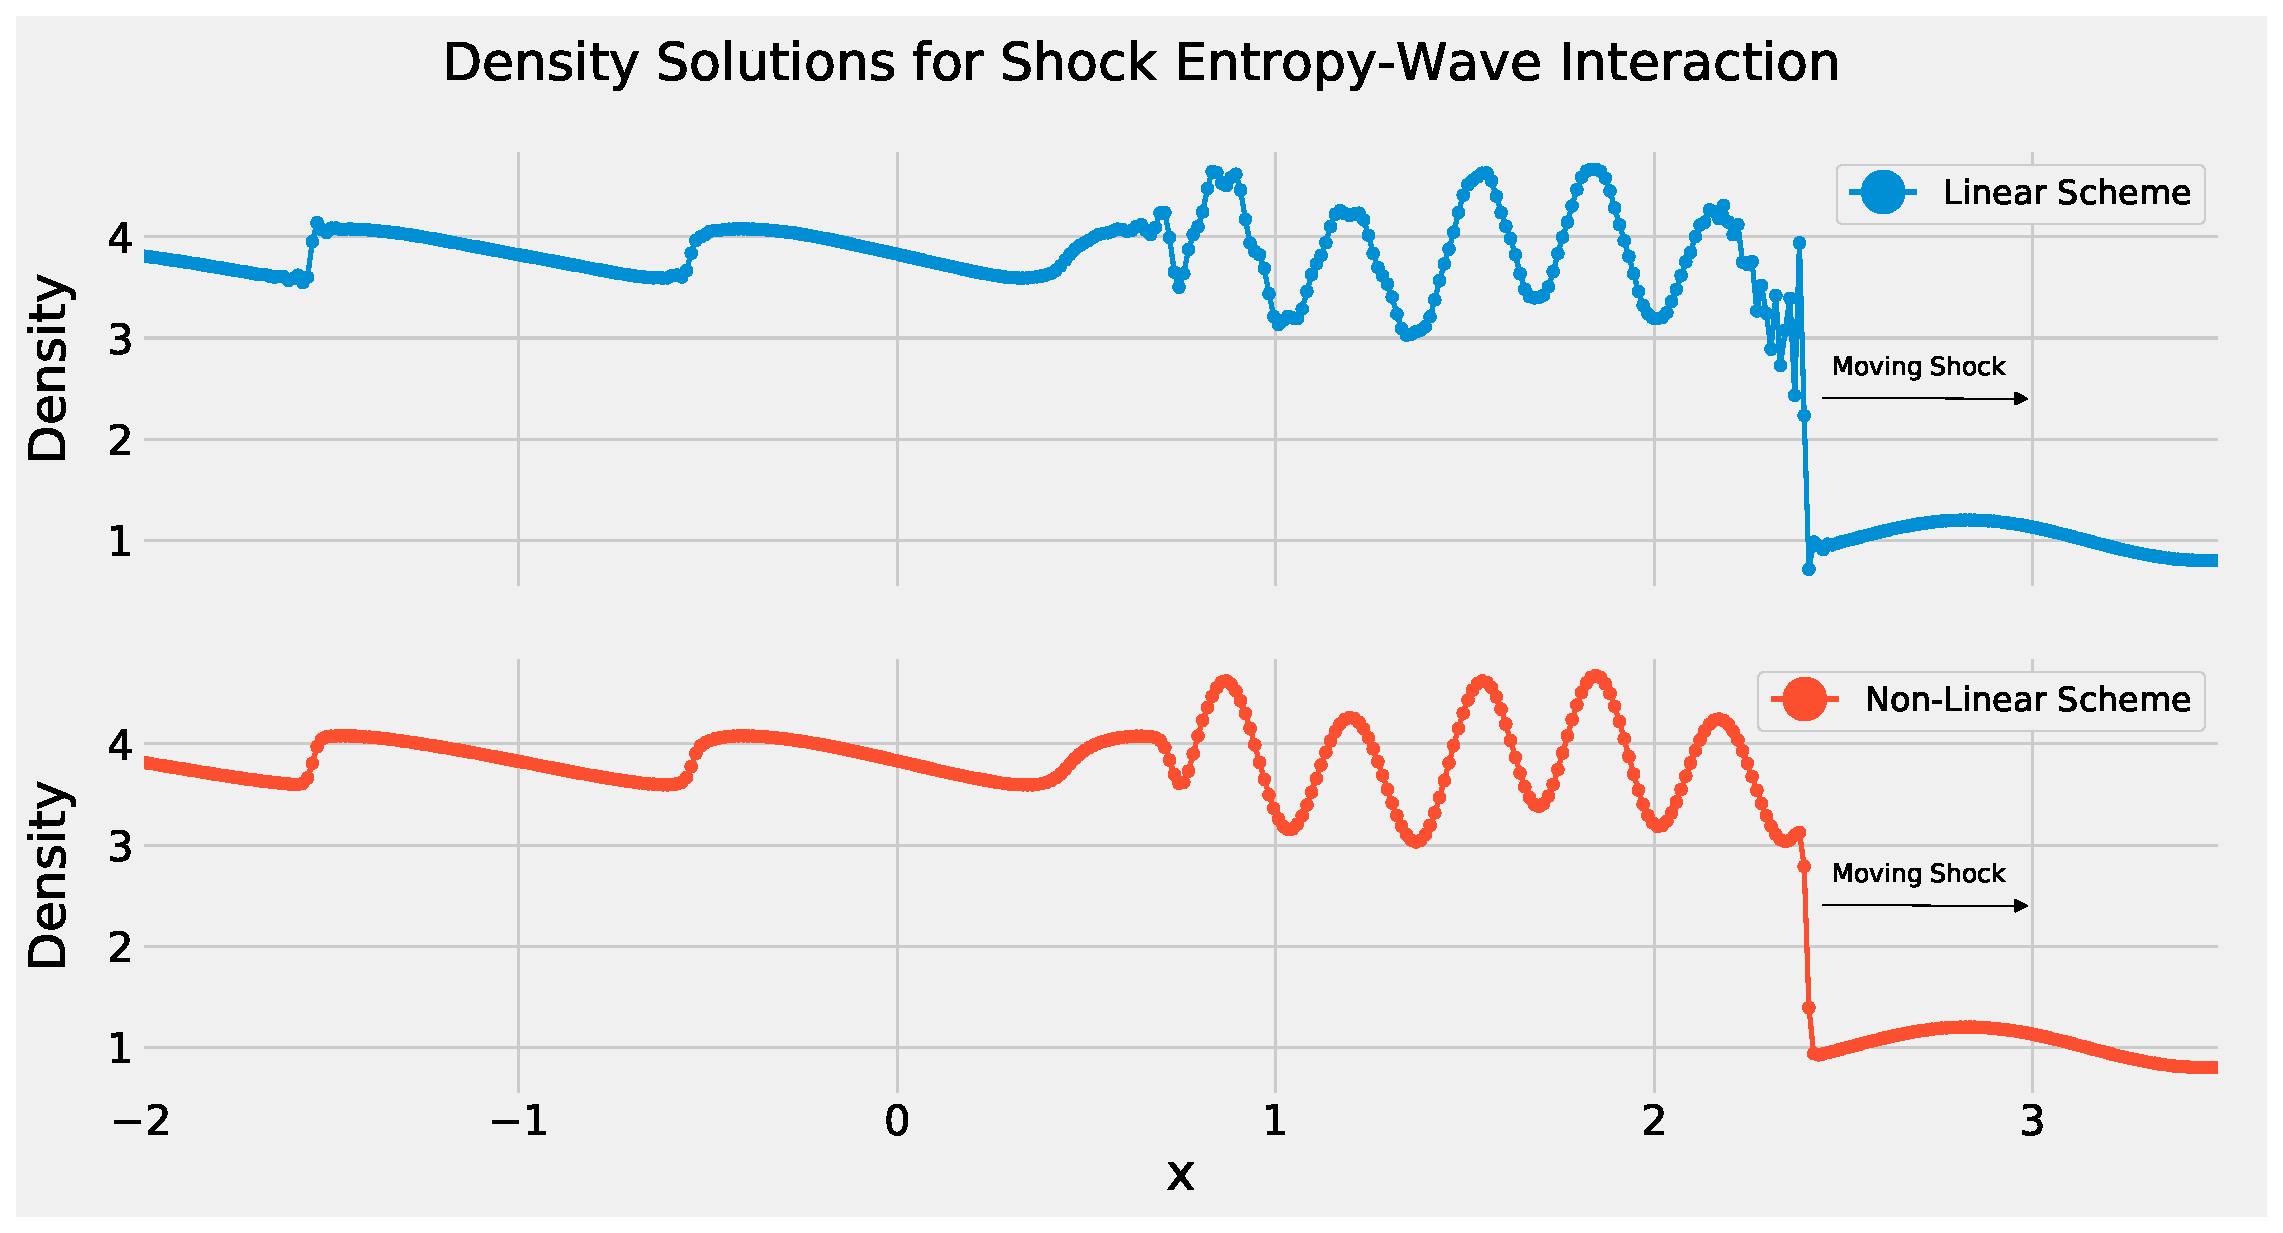
\includegraphics[scale=0.25]{DensitySolutions.eps}\caption{Comparison of linear and non-linear schemes for shock-entropy wave interaction problem}
      \label{fig:ShockEntropy}
    \end{figure}
\end{frame}

\begin{frame}{Non-linear schemes also have issues}
  Explain positivity (show graphic?)
\end{frame}

\begin{frame}{Go through positivity process}
 math
\end{frame}

\begin{frame}{Positivity is good for Burgers equation}
  
\end{frame}


\begin{frame}{Positivity is even better for Euler}
  show several plots - demos to illustrate this.
\end{frame}


\begin{frame}{Motivation - Non-Linear Schemes}
\textbf{Why Non-Linear Schemes?}
\begin{itemize}
\item High order Finite Difference schemes suffer from spurious oscillations near discontinuities
\item Non-linear methods attenuate oscillations by utilizing a feedback loop to adjust the solution scheme near discontinuities
\begin{itemize}
\item[--] High order solution is retained in smooth regions 
\item[--] First order, non-oscillatory solution is obtained in discontinuous regions
\end{itemize}
\end{itemize}
\end{frame}



\begin{frame}{Non-linear Scheme Comparison}
The figure below shows two high-order solutions to a moving shock problem.  The linear scheme gives un-physical oscillations near the shock and other sharp features in the solution;  these issues are remedied by the non-linear scheme.
\begin{figure}[H]
\centering
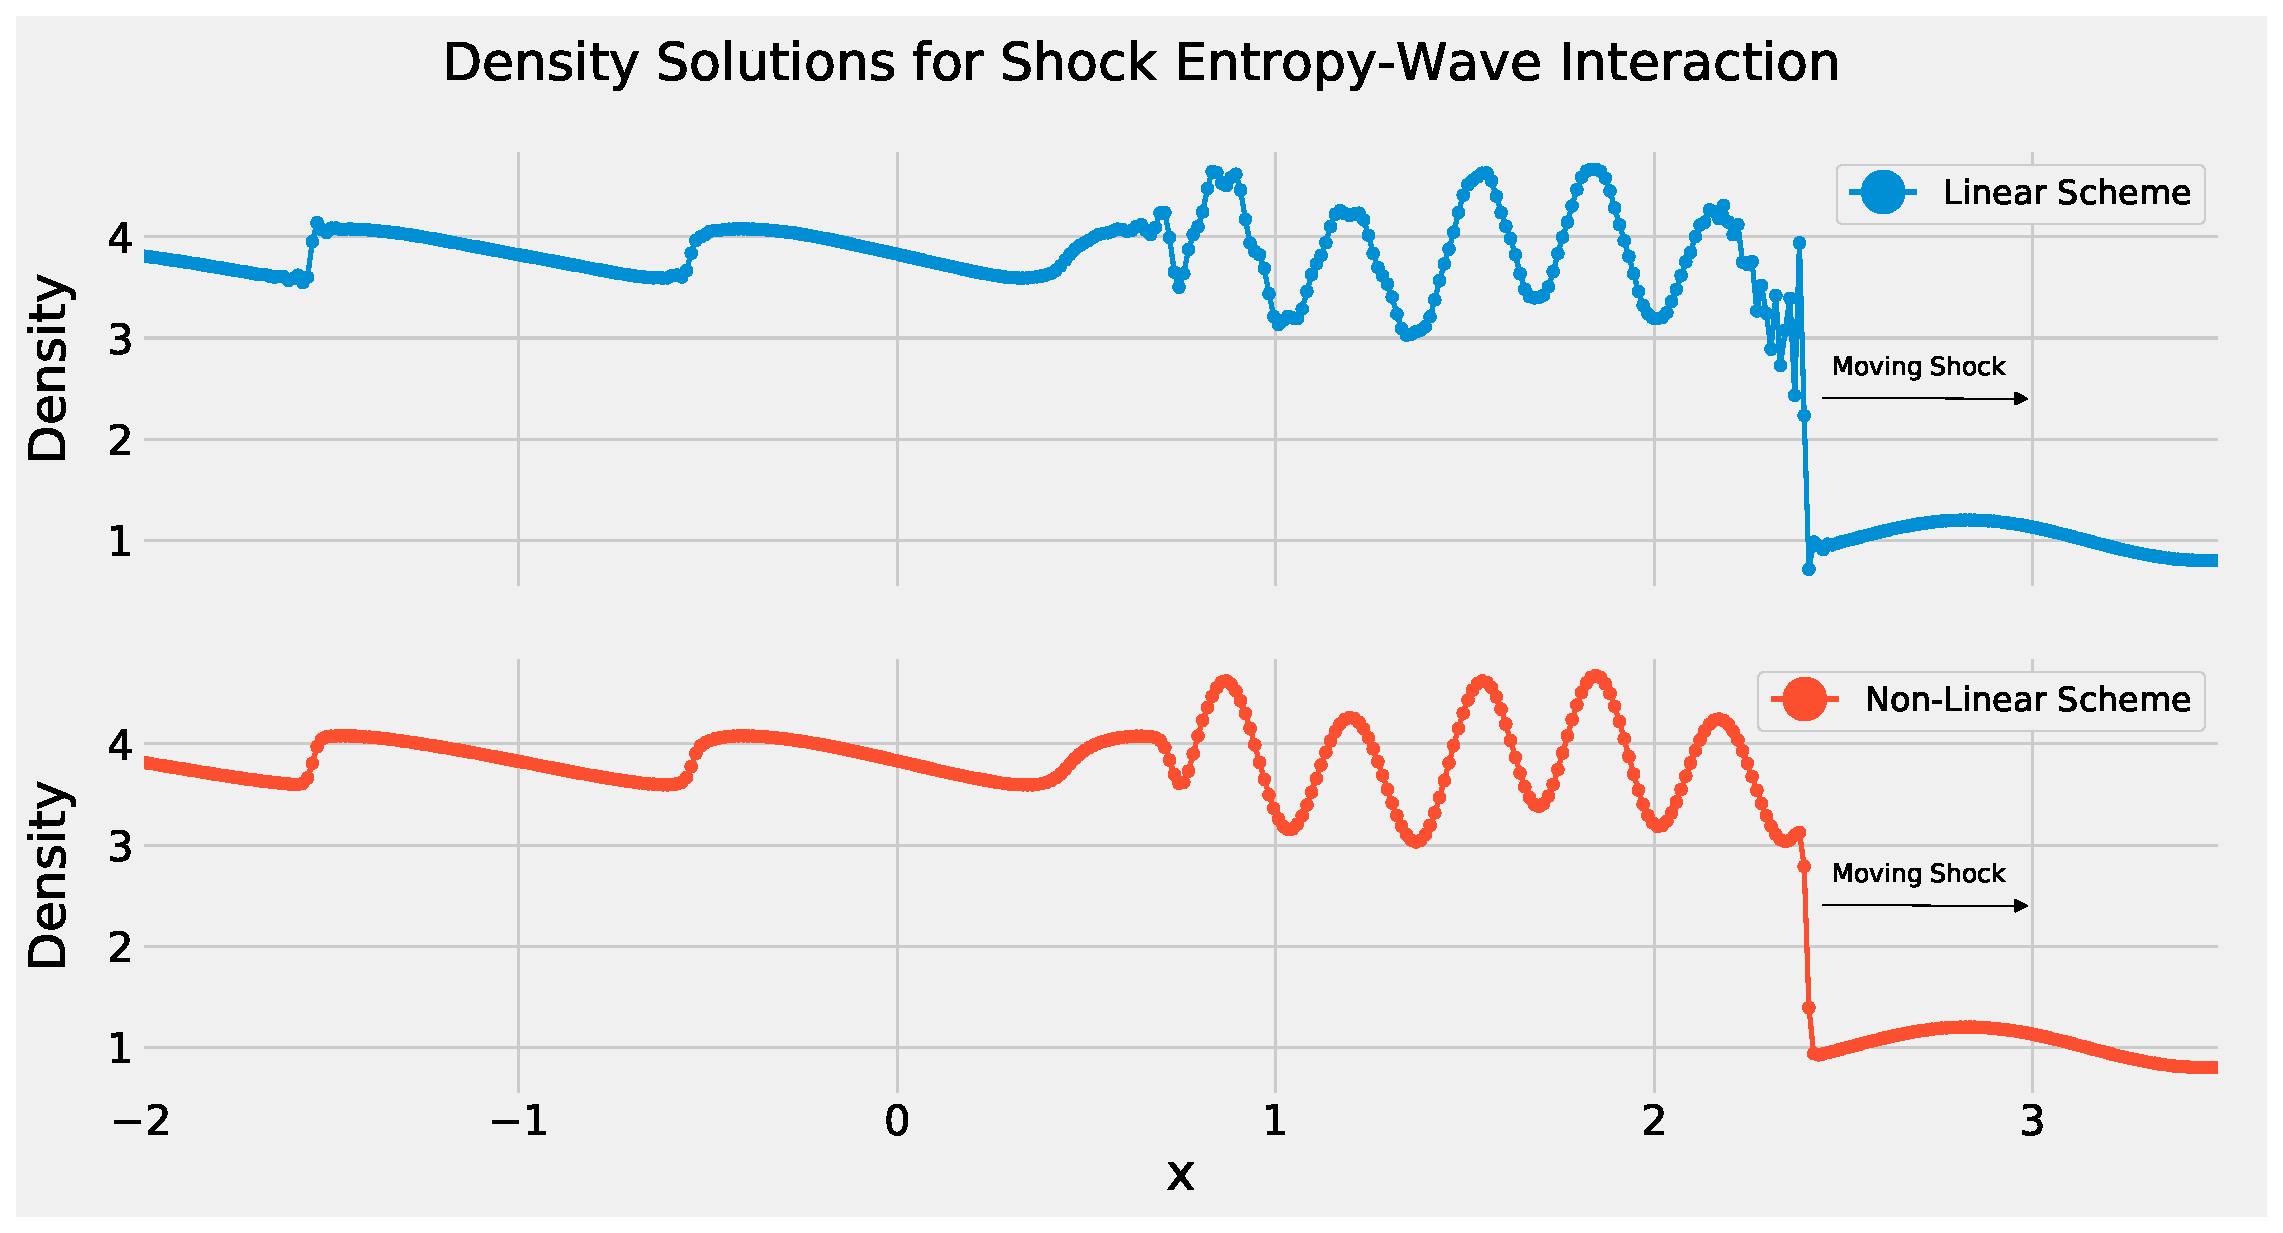
\includegraphics[scale=0.25]{DensitySolutions.eps}\caption{Comparison of linear and non-linear schemes for shock-entropy wave interaction problem}
  \label{fig:BurgersZoom}
\end{figure}
\end{frame}


\begin{frame}{Research Goals}
  The overall goals of this project are as follows:
  \begin{itemize}
  \item Implement Dr. Shahbazi's proposed primitive variable based WENO scheme \cite{Shahbazi} for $9^{\text{th}}$ order and higher
  \item Enforce positivity preservation for density and pressure
  \begin{itemize}
  \item[--] Generalize methods of Xiong et al \cite{Positivity2014} to primitive variable based WENO scheme.
  \end{itemize}
  \item Extend to multi-phase model
  \begin{itemize}
  \item[--] Four equation model of Saurel et al \cite{FourEquationModel}
  \item[--] Five equation model \cite{FiveEquationModel}
  \end{itemize}
  \item Extend to 2D
  \end{itemize}
\end{frame}

\section{High Level Description of Method}

\begin{frame}{Euler Equations of Gas Dynamics}
To demonstrate the mechanisms of a non-linear scheme, consider the three-dimensional Euler Equations of gas dynamics:
\begin{align}
\frac{\partial \rho}{\partial t}+\frac{\partial}{\partial x_j}[\rho v_j] &=0\label{eq:MassBalance}\\
\frac{\partial}{\partial t}[\rho v_i]+\frac{\partial}{\partial x_j}[\rho v_iv_j+p\delta_{ij}]&=0\label{eq:MomentaBalance}\\
\frac{\partial}{\partial t}[\rho(e+\tfrac{v_jv_j}{2})]+\frac{\partial}{\partial x_i}[(\rho e+\tfrac{\rho v_jv_j}{2} +p)v_i]&=0\label{eq:EnergyBalance}
\end{align}

where $e$ is the specific internal energy. In addition to these three equations, an additional property relation (e.g. Ideal Gas Law) is utilized in order to obtain a solvable system. 
\end{frame}

% Add gamma for air.. Euler Equations for liquid and gasses

\begin{frame}{Numerical Interpretation of Euler System}
Each one of the Euler Equations is just a conservation law of the form:
\begin{equation}
	\frac{\partial u}{\partial t}=-\frac{\partial}{\partial x}[f(u)]\label{eq:ConservationLaw}
\end{equation}
 enforced upon mass, momentum, and energy, respectively. We define a vector of conserved variables as: $$\textbf{u}=[\rho,\rho v,\rho(e+\tfrac{v^2}{2})]^T$$ and the flux of the conserved variables as:
\begin{equation}
	\textbf{f} = [\rho v, \rho v^2 + p, (\rho e +\frac{\rho v^2}{2}+p)v]^T\label{eq: Flux Functions}
\end{equation}

Finally, we can define the primitive variables as the quantities from which the conservation variables are constructed

\begin{equation}
\textbf{u}_p=[\rho,v,p]^T
\end{equation}

\end{frame}


\begin{frame}{WENO Overview}
The Weighted Essentially Non-Oscillatory (WENO) method is non-linear scheme designed to achieve non-oscillatory behavior near discontinuities while preserving high-order accuracy in smooth regions \cite{Jiang96}.  The method involves forming $r$ Lagrange polynomial reconstructions on $k_s\in[0,r-1]$ stencils surrounding a point $x_i$.
\begin{equation}
P_{r,k_s}(x_{i+\tfrac{1}{2}}) = \sum_{q=0}^{q=r-1}a_{r,k_s,q}u_{i-k_s+q}\label{eq:PolynomialReconstruction}
\end{equation}
These $r^{th}$ order polynomial approximations are then summed as a convex combination
\begin{equation}
P_{WENO, 2r-1}(x_{i+\frac{1}{2}})=\sum_{k_s=0}^{k_s=r-1}\omega_{r,k_s,i+\frac{1}{2}}P_{r,k_s}(x_{i+\tfrac{1}{2}})\label{eq:WenoEquation}
\end{equation}
where the non-linear weights $\omega_{r,k_s,i+\frac{1}{2}}$ are calculated using a smoothness indicator function such that any smooth sub-stencil is assigned an optimal weight while the contribution of any oscillatory sub-stencil goes to zero.  Thus, when all sub-stencils contain smooth approximations, the overall reconstruction will be of order $2r-1$.

\end{frame}

\begin{frame}{Traditional Flux Based Approach}
Traditionally, the WENO reconstruction process has been performed on the flux functions \eqref{eq: Flux Functions}.  This allows for the right hand side of a conservation law to be expressed exactly as:
\begin{equation}
\frac{\partial}{\partial	x}[f(u)]\bigg|_{x_i}=\frac{h(u_{i+1/2}) - h(u_{i-1/2})}{\Delta x} \label{eq: Traditional Derivative}
\end{equation}
where $h$ is defined to be some function that gives $f(u(x))$ when averaged over the interval $x\in[x-\frac{1}{2}\Delta x, x+\frac{1}{2}\Delta x]$, that is:
\begin{equation}
f(u(x))=\frac{1}{\Delta x} \int_{x-\frac{1}{2}\Delta x}^{x+\frac{1}{2}\Delta x}h(u(\xi))d\xi
\end{equation}
Since, $f(u(x_i))$ is known, the values $h(u_{i\pm1/2})\approx P_{WENO, 2r-1}(x_{i+\frac{1}{2}})$ can be approximated using the WENO scheme to yield a high order approximation to the spatial derivative term in the conservation law.  However, as shown by Shahbazi \cite{Shahbazi}, this approach can fail to preserve the non-oscillatory property for certain multi-fluid flow problems.  To combat this, a new method based upon the WENO reconstruction of primitive variables was proposed.
\end{frame}


\begin{frame}{Primitive Variable Reconstruction Approach}
The key difference between the traditional WENO method and the scheme proposed by Shahbazi \cite{Shahbazi} lies in how the spatial derivatives are calculated.  In the traditional approach, the derivatives are calculated using the WENO reconstruction directly on the flux functions.   In the new method, the derivatives are approximated to order $2r$ by performing the WENO reconstruction on the primitive variables and then forming the flux functions directly from these approximated values.  Here, the derivative term is calculated as:     

\begin{equation}
h\frac{\partial f}{\partial x}\bigg|_{x_i}\approx (\hat{f}_{i+1/2}-\hat{f}_{i-1/2}) = \sum_{q=0}^{q=r}d_q(f^{WENO}_{i+q-1/2}-f^{WENO}_{i-q-1/2})
\label{eq: derivative definition}
\end{equation}  

With Equation \ref{eq: derivative definition} giving a high order approximation for the right hand side of each governing equation, a High-order Runge-Kutte method can be utilized to integrate in time. 

\end{frame}


\begin{frame}[standout]
  Thank You
\end{frame}

\appendix

\begin{frame}[allowframebreaks]{References}

  \bibliography{references.bib}
  \bibliographystyle{abbrv}

\end{frame}


\end{document}